\caulc
%%%=============EX_1=============%%%
\begin{ex}%[1D2N2-4]%[TDMZZ05]%[Mui Doan]
	Cho cấp số cộng $(u_n)$ có $u_1=1$ và $d=2$. Giá trị của $u_{11}$ bằng
	\choice
	{\True $21$}
	{$23$}
	{$3$}
	{$12$}
	\loigiai{
		Ta có $u_{11}=u_1+10d=1+10\cdot 2=21$.
	}
\end{ex}
%%%=============================%%%

%%%=============EX_2=============%%%
\begin{ex}%[1D6H4-2]%[TDMZZ05]%[Huỳnh Trí Thiện]
	Nghiệm của phương trình $2^{x-1}=8$ là
	\choice
	{$x=3$}
	{\True $x=4$}
	{$x=5$}
	{$x=6$}
	\loigiai{
		Ta có $2^{x-1} = 8 \Leftrightarrow 2^{x-1} = 2^3 \Leftrightarrow x - 1 = 3 \Leftrightarrow x = 4$.\\
		Vậy nghiệm của phương trình là $x=4$.
	}
\end{ex}
%%%=============================%%%

%%%=============EX_3=============%%%
\begin{ex}%[1D6H4-3]%[TDMZZ05]%[Chu Hà]
	Tập nghiệm của bất phương trình $\log_{0{,}2}(x-2)>-1$ là
	\choice
	{$(7;+\infty)$}
	{$\{2;7\}$}
	{\True $(2;7)$}
	{$(-\infty;2)$}
	\loigiai{
		Điều kiện xác định là $x-2>0 \Leftrightarrow x>2$.\\
		Ta có
		$\log_{0{,}2}(x-2)>-1 \Leftrightarrow x-2<(0{,}2)^{-1}\Leftrightarrow x-2<5 \Leftrightarrow x<7$.\\
		Kết hợp với điều kiện $x>2$, ta được $2<x<7$.\\
		Vậy tập nghiệm là $(2;7)$.
	}
\end{ex}
%%%=============================%%%

%%%=============EX_4=============%%%
\begin{ex}%[1H8H2-3]%[TDMZZ05]%[Nguyễn Tấn Linh]
	Cho hình chóp $S. ABCD$ có đáy $ABCD$ là hình chữ nhật (nhưng không phải hình vuông), có cạnh bên $SA$ vuông góc với mặt phẳng đáy $(ABCD)$. Đáp án cho nhận xét \textbf{sai} là
	\choice
	{$SA \perp BD$}
	{$(SAB) \perp (ABCD)$}
	{$SB \perp BC$}
	{\True $BD \perp SC$}
	\loigiai{
		\immini{
			Ta xét các phương án:
			\begin{itemize}
				\item Vì $SA \perp (ABCD)$ và $BD \subset (ABCD)$ nên $SA \perp BD$.
				\item Vì $\heva{& SA \perp (ABCD)\\ & SA \subset (SAB)} \Rightarrow (SAB) \perp (ABCD)$.
				\item Ta có $\heva{& BC \perp AB \text{ (do $ABCD$ là hình chữ nhật)}\\ & BC \perp SA \text{ (do $SA \perp (ABCD)$)}} \Rightarrow BC \perp (SAB) \Rightarrow BC \perp SB$.
				\item Giả sử $BD \perp SC$. Kết hợp với $BD \perp SA$ ta suy ra $BD \perp (SAC) \Rightarrow BD \perp AC$. Điều này xảy ra khi và chỉ khi đáy $ABCD$ là hình vuông (trái với giả thiết của bài toán).
			\end{itemize}
		}
		{
			\begin{tikzpicture}[line join=round,line cap=round,font=\footnotesize,scale=.7]
				\coordinate (B) at (0,0);
				\coordinate (A) at (1.5,1.2);
				\coordinate (C) at (4,0);
				\coordinate (D) at ($(C)-(B)+(A)$);
				\coordinate (S) at ($(A)+(90:3.5)$);
				\draw (B)--(C)--(D)--(S)--cycle (S)--(C);
				\draw[dashed] (A)--(D) (S)--(A)--(B) (A)--(C) (B)--(D);
				\draw ($ (A)!5pt!(D)$)--($(A)!2!($($(A)!5pt!(D)$)!.5!($(A)!5pt!(S)$)$)$)--($(A)!5pt!(S)$);
				\draw ($ (A)!5pt!(B)$)--($(A)!2!($($(A)!5pt!(B)$)!.5!($(A)!5pt!(S)$)$)$)--($(A)!5pt!(S)$);
				\foreach \diem/\goc in {A/160,B/-90,C/-90,D/0,S/90} \fill[black](\diem) circle (1pt) ($(\diem)+(\goc:3mm)$) node{$\diem$};
			\end{tikzpicture}
		}
	}
\end{ex}
%%%=============================%%%

%%%=============EX_5=============%%%
\begin{ex}%[2D1N4-1]%[TDMZZ05]%[Phạm Hải Dương]
	Tổng số đường tiệm cận của đồ thị hàm số $y = \dfrac{x^2 - 4x + 3}{x - 1}$ là
	\choice
	{$2$}
	{\True $1$}
	{$3$}
	{$0$}
	\loigiai{
		Tập xác định $\mathscr{D} = \mathbb{R} \setminus \{1\}$.\\
		Ta có $y = \dfrac{x^2 - 4x + 3}{x - 1} = \dfrac{(x - 1)(x - 3)}{x - 1} = x - 3$ với mọi $x \neq 1$.\\
		Ta có $\lim\limits_{x \to 1} y = \lim\limits_{x \to 1} (x - 3) = -2$. Nên đồ thị hàm số không có tiệm cận đứng.\\
		Mặt khác $\lim\limits_{x \to +\infty} y = \lim\limits_{x \to +\infty} (x - 3) = +\infty$ và $\lim\limits_{x \to -\infty} y = \lim\limits_{x \to -\infty} (x - 3) = -\infty$. Đồ thị hàm số không có tiệm cận ngang.\\
		Ta có $\lim\limits_{x \to \pm\infty} \big[y -(x-3)\big]=0$ nên đường thẳng $y = x - 3$ là tiệm cận xiên của đồ thị hàm số.
	}
\end{ex}
%%%=============================%%%

%%%=============EX_6=============%%%
\begin{ex}%[1D5H1-3]%[TDMZZ05]%[Nguyễn Sơn Thành]
	Cho ba mẫu số liệu ghép nhóm $M_1$, $M_2$ với bảng tần số ghép nhóm như sau
	\begin{center}
		Nhóm $M_1$
		\begin{tabular}{|c|c|c|c|c|c|c|}
			\hline
			Nhóm & $\left[5;7\right)$ &$\left[7;9\right)$ &$\left[9;11\right)$ &$\left[11;13\right)$ &$\left[13;15\right)$ &$\left[15;17\right)$ \\
			\hline
			Tần số $M_1$ & $3$ & $5$ & $6$ & $4$ & $6$ & $9$ \\
			\hline
		\end{tabular}
	\end{center}
	
	\begin{center}
		Nhóm $M_2$
		\begin{tabular}{|c|c|c|c|c|c|c|}
			\hline
			Nhóm & $\left[5;7\right)$ &$\left[7;9\right)$ &$\left[9;11\right)$ &$\left[11;13\right)$ &$\left[13;15\right)$ &$\left[15;17\right)$ \\
			\hline
			Tần số $M_2$ & $3$ & $5$ & $6$ & $4$ & $6$ & $12$ \\
			\hline
		\end{tabular}
	\end{center}
	
	\begin{center}
		Nhóm $M_3$
		\begin{tabular}{|c|c|c|c|c|c|c|}
			\hline
			Nhóm & $\left[5;7\right)$ &$\left[7;9\right)$ &$\left[9;11\right)$ &$\left[11;13\right)$ &$\left[13;15\right)$ &$\left[15;17\right)$ \\
			\hline
			Tần số $M_3$ & $8$ & $5$ & $6$ & $4$ & $6$ & $9$ \\
			\hline
		\end{tabular}
	\end{center}
	Hãy so sánh số trung bình cộng $\overline{x}_1$, $\overline{x}_2$, $\overline{x}_3$ của ba mẫu số liệu $M_1$, $M_2$, $M_3$?
	\choice
	{$\overline{x}_3 > \overline{x}_1 > \overline{x}_2$}
	{$\overline{x}_1 < \overline{x}_2 < \overline{x}_3$}
	{$\overline{x}_1 = \overline{x}_2 > \overline{x}_3$}
	{\True $\overline{x}_3 < \overline{x}_1 < \overline{x}_2$}
	\loigiai{
		Ta có
		\begin{itemize}
			\item $\overline{x}_1 = \dfrac{3 \cdot 6 + 5 \cdot 8 + 6 \cdot 10 + 4 \cdot 12 + 6 \cdot 14 + 9 \cdot 16}{33} = \dfrac{394}{33} \approx 11{,}94$.
			\item $\overline{x}_2 = \dfrac{3 \cdot 6 + 5 \cdot 8 + 6 \cdot 10 + 4 \cdot 12 + 6 \cdot 14 + 12 \cdot 16}{36} = \dfrac{442}{36} = \dfrac{221}{18} \approx 12{,}28$.
			\item $\overline{x}_3 = \dfrac{8 \cdot 6 + 5 \cdot 8 + 6 \cdot 10 + 4 \cdot 12 + 6 \cdot 14 + 9 \cdot 16}{38} = \dfrac{424}{38} = \dfrac{212}{19} \approx 11{,}16$.
		\end{itemize}
		Vậy $\overline{x}_3 < \overline{x}_1 < \overline{x}_2$.
		
		\textbf{Cách khác:}\\
		Giá trị đại diện của các nhóm lần lượt là $6; 8; 10; 12; 14; 16$.
		\begin{itemize}
			\item So sánh $M_1$ và $M_2$: $M_2$ có tần số ở nhóm có giá trị đại diện lớn nhất ($16$) cao hơn $M_1$, trong khi các nhóm khác giữ nguyên, suy ra $\overline{x}_2 > \overline{x}_1$.
			\item So sánh $M_1$ và $M_3$: $M_3$ có tần số ở nhóm có giá trị đại diện nhỏ nhất ($6$) cao hơn $M_1$, trong khi các nhóm khác giữ nguyên, suy ra $\overline{x}_3 < \overline{x}_1$.
		\end{itemize}
		Vậy $\overline{x}_3 < \overline{x}_1 < \overline{x}_2$.
	}
\end{ex}
%%%=============================%%%

%%%=============EX_7=============%%%
\begin{ex}%[2H2N1-2]%[TDMZZ05]%[Bồ Văn Hậu]
	\immini[thm]{Cho hình hộp $ABCD. A'B'C'D'$. Khẳng định nào sau đây là \textbf{đúng}?
		\choice
		{$\overrightarrow{AC}+\overrightarrow{CB'}+\overrightarrow{B'B}=\overrightarrow{AB'}$}
		{$\overrightarrow{AA'}+\overrightarrow{BB'}+\overrightarrow{DD'}=\overrightarrow{AB'}$}
		{\True $\overrightarrow{AD}+\overrightarrow{DB}+\overrightarrow{DD'}=\overrightarrow{AB'}$}
		{$\overrightarrow{AB}+\overrightarrow{BC'}+\overrightarrow{CB'}=\overrightarrow{AB'}$}
	}{
		\begin{tikzpicture}[line cap=round, line join=round, font=\footnotesize, >=stealth, scale=0.6]
			\path 
			(0,0) coordinate (A)
			(5,0) coordinate (D)
			(-2,-2) coordinate (B)
			($(D) - (A) + (B)$) coordinate (C)
			($(A) + (0.5,3)$) coordinate (A')
			($(B) + (0.5,3)$) coordinate (B')
			($(C) + (0.5,3)$) coordinate (C')
			($(D) + (0.5,3)$) coordinate (D')
			;
			\draw[dashed] (A')--(A) (B)--(A)--(D);
			\draw (A')--(B')--(C')--(D')--cycle (D')--(D)--(C) (B')--(B)--(C)--(C')--cycle;
			\foreach \i/\r in {A/150, B/-135, C/-45, D/0, A'/105, B'/180, C'/-45, D'/45}{
				\filldraw[black] (\i) circle (1pt);
				\node at ($(\i) + (\r:4mm)$) {$\i$};
			}
	\end{tikzpicture}}
	\loigiai{
		Ta có $ABCD. A'B'C'D'$ là hình hộp nên $\overrightarrow{DD'}=\overrightarrow{BB'}$, suy ra \[\overrightarrow{AD}+\overrightarrow{DB}+\overrightarrow{DD'}=\overrightarrow{AB}+\overrightarrow{BB'}=\overrightarrow{AB'}.\]
	}
\end{ex}
%%%=============================%%%

%%%=============EX_8=============%%%
\begin{ex}%[2D4H1-3]%[TDMZZ05]%[Lê Phúc]
	Nguyên hàm của hàm số $y=2\cos^2\left(\dfrac{\pi-x}{2}\right)$ là
	\choice
	{$\dfrac{1}{3}\cos^3\left(\dfrac{\pi-x}{2}\right)+C$}
	{$x-\cos x+C$}
	{$x+\sin x+C$}
	{\True $x-\sin x+C$}
	\loigiai{
		Ta có $y=\cos\left[2\left(\dfrac{\pi-x}{2}\right)\right]+1=\cos\left(\pi-x\right)+1=-\cos x+1$.\\
		Suy ra $\displaystyle\int y \mathrm{\,d}x=\displaystyle\int (-\cos x+1) \mathrm{\,d}x=-\sin x+x+C$.
	}
\end{ex}
%%%=============================%%%

%%%=============EX_9=============%%%
\begin{ex}%[2H2N2-2]%[TDMZZ05]%[Trần Văn Thiện]
	Trong không gian $Oxyz$ cho điểm $A(2;5;-3)$. Điểm đối xứng với $A$ qua mặt phẳng $(Oxz)$ có tọa độ là
	\choice
	{\True $(2;-5;-3)$}
	{$(2;5;-3)$}
	{$(2;5;3)$}
	{$(-2;-5;-3)$}
	\loigiai{
		Hình chiếu của điểm $A(2;5;-3)$ lên mặt phẳng $(Oxz)$ là điểm $H(2;0;-3)$.\\
		Điểm $A'$ đối xứng với $A$ qua mặt phẳng $(Oxz)$ nên $H$ là trung điểm của $AA'$. Do đó tọa độ $A'(2; -5;-3)$.
	}
\end{ex}
%%%=============================%%%

%%%=============EX_10=============%%%
\begin{ex}%[2D4H3-1]%[TDMZZ05]%[Đình Nguyên]
	Diện tích hình phẳng giới hạn bởi các đường $y=x^2-1$, $y=0$, $x=0$, $x=2$ là
	\choice
	{$\dfrac{8}{3}$}
	{$\dfrac{4}{3}$}
	{\True $2$}
	{$1$}
	\loigiai{
		Phương trình hoành độ giao điểm của đường cong $y=x^2-1$ và trục hoành $y=0$ là
		$x^2-1=0 \Leftrightarrow x=\pm 1$.\\
		Trên đoạn $[0;2]$, phương trình có nghiệm $x=1$.\\
		Diện tích hình phẳng cần tìm là
		\begin{eqnarray*}
			S &=& \displaystyle\int\limits_0^2 \left|x^2-1\right| \mathrm{\,d}x = \displaystyle\int\limits_0^1 \left|x^2-1\right| \mathrm{\,d}x + \displaystyle\int\limits_1^2 \left|x^2-1\right| \mathrm{\,d}x \\
			&=& \displaystyle\int\limits_0^1 (1-x^2) \mathrm{\,d}x + \displaystyle\int\limits_1^2 (x^2-1) \mathrm{\,d}x = \left.\left(x-\dfrac{x^3}{3}\right)\right|_0^1 + \left.\left(\dfrac{x^3}{3}-x\right)\right|_1^2 \\
			&=& \dfrac{2}{3} + \dfrac{4}{3} = 2.
		\end{eqnarray*}
	}
\end{ex}
%%%=============================%%%

%%%=============EX_11=============%%%
\begin{ex}%[2D1H2-1]%[TDMZZ05]%[Huynh Quốc Đạt]
	Đồ thị hàm số $y = x^3 - 6x^2 + 9x - 2\,026$ có hai điểm cực trị cách nhau một đoạn
	\choice
	{$2\sqrt{3}$}
	{$4$}
	{$3\sqrt{2}$}
	{\True $2\sqrt{5}$}
	\loigiai{
		Ta có $y' = 3x^2 - 12x + 9$.\\
		Cho $y' = 0 \Leftrightarrow 3x^2 - 12x + 9 = 0 \Leftrightarrow \hoac {&x = 1 \Rightarrow y = -2\,022 \\ &x = 3 \Rightarrow y = -2\,026.}$\\
		Hai điểm cực trị của đồ thị hàm số là $A(1; -2\,022)$ và $B(3; -2\,026)$.\\
		Độ dài đoạn thẳng $AB$ là
		\[AB = \sqrt{(3-1)^2 + \left(-2\,026 - (-2\,022)\right)^2} = \sqrt{2^2 + (-4)^2} = \sqrt{20} = 2\sqrt{5}.\]
		Vậy hai điểm cực trị cách nhau một đoạn bằng $2\sqrt{5}$.
	}
\end{ex}
%%%=============================%%%

%%%=============EX_12=============%%%
\begin{ex}%[2H5N1-3]%[TDMZZ05]%[Nguyễn Trí Minh Tuấn]
	Trong không gian $Oxyz$, cho hai điểm $A(1;2;3)$, $B(3;3;4)$. Mặt phẳng đi qua gốc tọa độ và vuông góc với đường thẳng $AB$ là
	\choice
	{$2x+y+z-2=0$}
	{\True $2x+y+z=0$}
	{$x+2y+3z=0$}
	{$3x+3y+4z=0$}
	\loigiai{
		Ta có $\overrightarrow{AB}=(3-1; 3-2; 4-3)=(2;1;1)$.\\
		Vì mặt phẳng vuông góc với đường thẳng $AB$ nên một vectơ pháp tuyến của mặt phẳng là
		$\overrightarrow{n}=\overrightarrow{AB}=(2;1;1)$.\\
		Do đó mặt phẳng có dạng $2x+y+z+d=0$.\\
		Mặt phẳng đi qua gốc tọa độ $O(0;0;0)$ nên $2\cdot 0+0+0+d=0 \Rightarrow d=0$.\\
		Vậy phương trình mặt phẳng là $2x+y+z=0$.
	}
\end{ex}
%%%=============================%%%

\cauds
%%%=============EX_13=============%%%
\begin{ex}%[2D4H3-1]%[TDMZZ05]%[Dương Công Tạo]
	Cho hàm số $y = f(x) = x^4 - 4x^2 + 3$ có đồ thị $(C)$.
	\choiceTF
	{$f'(x) = 4x^3 - 4x$}
	{\True $(C)$ có $1$ điểm cực đại và hai điểm cực tiểu}
	{\True Diện tích hình phẳng giới hạn bởi $(C)$ và trục $Ox$ bằng $4{,}7$ (\textit{làm tròn kết quả đến hàng phần mười})}
	{\True Ba điểm cực trị của $(C)$ tạo thành một tam giác có diện tích bằng $4\sqrt{2}$}
	\loigiai{
		\begin{itemchoice}
			\itemch Ta có $y = f(x) = x^4 - 4x^2 + 3$. Suy ra $f'(x) = 4x^3-8x$.
			\itemch Xét hàm số $y = f(x) = x^4 - 4x^2 + 3$.\\
			Tập xác định $\mathscr{D}=\mathbb{R}$.\\
			Ta có $f'(x) = 4x^3-8x=4x\left(x^2-2\right)$; $f'(x)=0\Leftrightarrow \hoac{&x=0\\&x=\pm\sqrt{2}.}$\\
			Bảng biến thiên
			\begin{center}
				
\begin{tikzpicture}[>=stealth]
					\tkzTabInit[nocadre=false,lgt=1.5,espcl=2,deltacl=0.6]{$x$/.7 ,$f'(x)$/.7,$f(x)$/2}
					{$-\infty$ , $-\sqrt{2}$ , $0$ , $\sqrt{2}$, $+\infty$}
					\tkzTabLine{ , -  ,0 , + , 0 , - , 0 , + , }
					\tkzTabVar{+/$+\infty$ , -/$-1$ , +/$0$ , -/$-1$ , +/$+\infty$}
				\end{tikzpicture}
			\end{center}
			Dựa vào bảng biến thiên, ta thấy đồ thị hàm số có $2$ điểm cực tiểu và $1$ điểm cực đại.
			\itemch Ta có $x^4-4x^2+3=0\Leftrightarrow\hoac{&x^2=1\\&x^2=3}\Leftrightarrow\hoac{&x=\pm 1\\&x=\pm\sqrt{3}.}$\\
			Khi đó, diện tích hình phẳng giới hạn bởi $(C)$ và trục $Ox$ là
			\begin{eqnarray*}
				S &=& \displaystyle\int\limits_{-\sqrt{3}}^{\sqrt{3}}\left|x^4-4x^2+3\right|\mathrm{\,d}x = 2\displaystyle\int\limits_{0}^{\sqrt{3}}\left|x^4-4x^2+3\right|\mathrm{\,d}x\\
				&=& 2\left[\displaystyle\int\limits_{0}^{1}\left(x^4-4x^2+3\right)\mathrm{\,d}x + \displaystyle\int\limits_{1}^{\sqrt{3}}\left(-x^4+4x^2-3\right)\mathrm{\,d}x\right] \\
				&=& 2\left[ \dfrac{28}{15} + \left(-\dfrac{9\sqrt{3}}{5} + 4\sqrt{3} - 3\sqrt{3}\right) - \left(-\dfrac{1}{5} + \dfrac{4}{3} - 3\right) \right] \\
				&=& 2\left[ \dfrac{56}{15} - \dfrac{4\sqrt{3}}{5} \right] \approx 4{,}7.
			\end{eqnarray*}
			\itemch Dựa vào bảng biến thiên trên ý b), ta thấy đồ thị hàm số đạt cực đại tại điểm $A(0;3)$, cực tiểu tại điểm $B\left(-\sqrt{2};-1\right)$ và $C\left(\sqrt{2};-1\right)$.\\
			Vì $AB=AC=3\sqrt{2}$ nên $\triangle ABC$ cân tại $A$ có $H(0;-1)$ là trung điểm $BC$ nên \[S_{ABC}=\dfrac{1}{2}\cdot AH\cdot BC=\dfrac{1}{2}\cdot 4\cdot 2\sqrt{2}=4\sqrt{2}.\]
		\end{itemchoice}
	}
\end{ex}
%%%=============================%%%

%%%=============EX_14=============%%%
\begin{ex}%[2D4H3-5]%[TDMZZ05]%[Hà Văn Hảo]
	Cho một vật bắt đầu chuyển động thẳng trên trục $Ox$ với đồ thị vận tốc theo thời gian như hình vẽ. Biết từ giây thứ $9$ đến giây thứ $15$ đồ thị vận tốc là đường hình sin có phương trình là $v(t)=a+b\sin \left(\dfrac{\pi}{3}t\right)$ m/s. Trong bài toán vận tốc tính theo m/s, quãng đường tính theo mét, thời gian tính theo giây.
	\begin{center}
		\begin{tikzpicture}[>=stealth, x=0.8cm, y=0.8cm, scale=0.8] 
			\draw[->] (0,0) -- (17,0) node[below] {$t\,(s)$};
			\draw[->] (0,0) -- (0,6) node[left] {$v(t)$};
			\node[below left] at (0,0) {$O$};
			\draw[blue, thick] (0,0) -- (4,3.5); 
			\draw[blue, thick] (4,3.5) -- (9,3.5);
			\draw[blue, thick, domain=9:15, samples=100] plot (\x, {3.5 - 1.5*sin((\x * pi / 3) r)}); 
			\draw[blue, thick] (15,3.5) -- (16.5,3.5);
			\draw[dashed] (4,0) node[below] {$4$} -- (4,3.5);
			\draw[dashed] (9,0) node[below] {$9$} -- (9,3.5);
			\draw[dashed] (12,0) node[below] {$12$} -- (12,3.5);
			\draw[dashed] (15,0) node[below] {$15$} -- (15,3.5)--(9,3.5);
			\draw[dashed] (0,3.5) node[left] {$3{,}5$} -- (9,3.5);
			\draw[dashed] (0,5) node[left] {$5$} -- (10.5,5) -- (10.5,0); 
			\draw[dashed] (0,2) node[left] {$2$} -- (13.5,2) -- (13.5,0); 
		\end{tikzpicture}
	\end{center}
	\choiceTF
	{\True Quãng đường vật đi được trong $4$ giây đầu tiên là $7$ m}
	{Biểu thức vận tốc của vật là $v(t)=\heva{&0{,}875t &&\text{nếu } 0 \le t < 4 \\ &3{,}5+1{,}5\sin \dfrac{\pi}{3}t &&\text{nếu } 9 \le t < 15}$}
	{\True Quãng đường vật đi được trong $15$ giây đầu tiên bằng $45{,}5$ m (\textit{làm tròn kết quả đến hàng phần mười khi tính theo đơn vị mét})}
	{\True Nếu tính theo mét (\textit{làm tròn kết quả đến hàng phần mười}) thì quãng đường vật đi được trong $11$ giây đầu tiên bằng $33{,}6$ m}
	\loigiai{
		\begin{itemchoice}
			\itemch Trong $4$ giây đầu, đồ thị là đoạn thẳng đi qua $O(0;0)$ và $\left(4; 3{,}5\right)$.\\
			Vận tốc $v(t) = \dfrac{3{,}5}{4}t = 0{,}875t$.\\
			Quãng đường $s_1 = \displaystyle\int_0^4 0{,}875t \mathrm{\,d}t = \dfrac{1}{2} \cdot 4 \cdot 3{,}5 = 7$ m.
			\itemch Dựa vào đồ thị:
			\begin{itemize}
				\item Với $0 \le t < 4$. Đồ thị là đường thẳng $v = kt$, đi qua $\left(4; 3{,}5\right) \Rightarrow k = \dfrac{3{,}5}{4} = 0{,}875$.
				\item Với $9 \le t < 15$. Đồ thị là đường hình sin $v(t) = a + b \sin\left(\dfrac{\pi}{3}t\right)$.\\
				Tại $t=9$, $v=3{,}5 \Rightarrow 3{,}5 = a + b\sin(3\pi) \Rightarrow a = 3{,}5$.\\
				Tại $t=10{,}5$, $v=5 \Rightarrow 5 = 3{,}5 + b \sin\left(\dfrac{\pi}{3} \cdot 10{,}5\right) \Rightarrow b = - 1{,}5$.
			\end{itemize}
			Vậy $v(t)=\heva{&0{,}875t &&\text{nếu } 0 \le t < 4 \\ &3{,}5-1{,}5\sin \dfrac{\pi}{3}t &&\text{nếu } 9 \le t < 15.}$
			\itemch Quãng đường vật đi được trong $15$ giây đầu tiên
			\allowdisplaybreaks
			\begin{eqnarray*}
				s_{15} &=& \displaystyle\int\limits_0^{15} v(t) \mathrm{\,d}t\\
				&=& \displaystyle\int\limits_0^4 0{,}875t \mathrm{\,d}t + \displaystyle\int\limits_4^9 3{,}5 \mathrm{\,d}t + \displaystyle\int\limits_9^{15} \left(3{,}5 - 1{,}5 \sin \dfrac{\pi}{3}t\right) \mathrm{\,d}t\\
				&=& 7 + 17{,}5 + \left. \left(3{,}5t + \dfrac{1{,}5 \cdot 3}{\pi} \cos \dfrac{\pi}{3}t\right) \right|_9^{15} \\
				&=& 7 + 17{,}5 + 21\\
				&=& 45{,}5 \, \text{m}.
			\end{eqnarray*}
			Vậy $s_{15}=45{,}5$ m.
			\itemch Quãng đường trong $11$ giây đầu tiên
			\allowdisplaybreaks
			\begin{eqnarray*}
				s_{11} &=& \displaystyle\int\limits_0^{11} v(t) \mathrm{\,d}t\\
				&=& \displaystyle\int\limits_0^4 0{,}875t \mathrm{\,d}t + \displaystyle\int\limits_4^9 3{,}5 \mathrm{\,d}t + \displaystyle\int\limits_9^{11} \left(3{,}5 - 1{,}5 \sin \dfrac{\pi}{3}t\right) \mathrm{\,d}t\\
				&=& 7 + 17{,}5 + \left. \left(3{,}5t + \dfrac{1{,}5 \cdot 3}{\pi} \cos \dfrac{\pi}{3}t\right) \right|_9^{11} \\
				&=& 24{,}5 + \left(38{,}5 + \dfrac{4{,}5}{\pi} \cos \dfrac{11\pi}{3}\right) - \left(31{,}5 + \dfrac{4{,}5}{\pi} \cos 3\pi\right)\\
				&=& 24{,}5 + 7 + \dfrac{4{,}5}{\pi} \left(\dfrac{1}{2} - (-1)\right) \\
				&=& 31{,}5 + \dfrac{6{,}75}{\pi} \approx 33{,}6 \, \text{m}.
			\end{eqnarray*}
			Vậy $s_{11}=33{,}6$ m.
		\end{itemchoice}
	}
\end{ex}
%%%=============================%%%

%%%=============EX_15=============%%%
\begin{ex}%[2D6V2-4]%[TDMZZ05]%[Vũ Hồng Toàn]
	Cho hai hộp I và II đựng những viên bi cùng kích thước và cùng khối lượng. Hộp I có $6$ bi đỏ và $4$ bi xanh, hộp II có $5$ bi đỏ và $3$ bi xanh. Tiến hành lấy ngẫu nhiên liên tiếp hai lần, mỗi lần lấy một viên bi từ hộp I theo quy tắc: nếu lấy được bi đỏ ta bỏ nó sang hộp II, nếu lấy được bi xanh thì ta bỏ trở lại hộp I. Sau đó lấy ngẫu nhiên một viên bi từ hộp II. Gọi $A$ là biến cố lấy được bi đỏ từ hộp II, $B$ là biến cố cả hai viên bi lấy ở hộp I đều được bỏ sang hộp II.
	\choiceTF
	{\True $\mathrm{P}(B) = \dfrac{1}{3}$}
	{\True $\mathrm{P}\left(A\mid B\right) = \dfrac{7}{10}$}
	{$\mathrm{P}(A) = 0{,}71$ (\textit{làm tròn kết quả đến hàng phần trăm})}
	{Xác suất để lấy được hai bi đỏ liên tiếp từ hộp I, nếu biết lấy được bi đỏ từ hộp II là $\dfrac{35}{93}$}
	\loigiai{
		\begin{itemchoice}
			\itemch Ta có
			\begin{itemize}
				\item Xác suất lần $1$ lấy được bi đỏ là $\mathrm{P}(R_1) = \dfrac{6}{10}=\dfrac{3}{5}$.
				\item Xác suất lần $2$ lấy được bi đỏ (sau khi lần $1$ đã lấy $1$ đỏ) là $\mathrm{P}\left(R_2 \mid R_1\right) = \dfrac{5}{9}$.
			\end{itemize}
			Áp dụng quy tắc nhân
			\[ \mathrm{P}(B) = \dfrac{3}{5} \cdot \dfrac{5}{9} = \dfrac{1}{3}. \]
			\itemch Khi biến cố $B$ đã xảy ra, hộp II đã nhận thêm $2$ bi đỏ từ hộp I.
			\begin{itemize}
				\item Số bi đỏ mới trong hộp II là $5 + 2 = 7$.
				\item Tổng số bi mới trong hộp II là $8 + 2 = 10$.
			\end{itemize}
			Vậy $\mathrm{P}\left(A\mid B\right) = \dfrac{7}{10}$.
			\itemch Ta xét các trường hợp sau
			\begin{enumerate}[\textbf{TH}.]
				\item ($H_1$): Chuyển $2$ bi đỏ sang hộp II ($B$ xảy ra).
				\[ \mathrm{P}(H_1) = \dfrac{1}{3}; \quad \mathrm{P}\left(A\mid H_1\right) = \dfrac{7}{10}. \]
				\item ($H_2$): Chuyển đúng $1$ bi đỏ sang hộp II.\\
				Có hai khả năng:
				\begin{itemize}
					\item (Đỏ - Xanh): $\dfrac{6}{10} \cdot \dfrac{4}{9} = \dfrac{4}{15}$.
					\item (Xanh - Đỏ): $\dfrac{4}{10} \cdot \dfrac{6}{10} = \dfrac{6}{25}$.
				\end{itemize}
				\[ \mathrm{P}(H_2) = \dfrac{4}{15} + \dfrac{6}{25} = \dfrac{38}{75}. \]
				\[ \mathrm{P}\left(A\mid H_2\right) = \dfrac{5+1}{8+1} = \dfrac{2}{3}. \]
				\item ($H_3$): Không chuyển bi đỏ nào ($2$ lần đều lấy bi xanh).
				\[ \mathrm{P}(H_3) = \dfrac{4}{10} \cdot \dfrac{4}{10} = \dfrac{4}{25}; \quad \mathrm{P}\left(A\mid H_3\right) = \dfrac{5}{8}. \]
			\end{enumerate}
			Vậy \[ \mathrm{P}(A) = \dfrac{1}{3} \cdot \dfrac{7}{10} + \dfrac{38}{75} \cdot \dfrac{2}{3}+ \dfrac{4}{25} \cdot \dfrac{5}{8}= \dfrac{302}{450} \approx 0{,}67.\]
			\itemch Áp dụng công thức Bayes
			\[ \mathrm{P}\left(B\mid A\right) = \dfrac{\mathrm{P}(B) \cdot \mathrm{P}\left(A\mid B\right)}{\mathrm{P}(A)} = \dfrac{\dfrac{1}{3} \cdot \dfrac{7}{10}}{\dfrac{302}{450}} = \dfrac{105}{302}.\]
		\end{itemchoice}
	}
\end{ex}
%%%=============================%%%

%%%=============EX_16=============%%%
\begin{ex}%[2H5C2-8]%[TDMZZ05]%[Văn Minh Thoại]
	\immini[thm]{
		Trong không gian $Oxyz$ đơn vị dài trên mỗi trục bằng $40$ cm, có một nguồn sáng điểm $S(3;2;6)$. Phương trình mặt thoáng của bể nước và đáy của bể nước lần lượt là $(\alpha)\colon z-3=0$ và $\left(\beta\right)\colon z=0$. Một tia sáng xuất phát từ điểm $S$, gặp mặt thoáng $(\alpha)$ tại điểm $I(1;0;3)$ (tia $SI$ nằm trong không khí), thì tia sáng (tia khúc xạ) sẽ bị đổi hướng (đi vào nước) tại $I$ và gặp đáy bể tại điểm $K$. Gọi $nn'$ là đường thẳng vuông góc với $(\alpha)$ tại $I$. Khi đó ta có $IK\subset\big(S,nn'\big)$ và có $\sin\widehat{KIn'}=\dfrac{3}{4}\sin\widehat{SIn}$.}{
		\begin{tikzpicture}[scale=0.9,line join=round,line cap=round,>=stealth,font=\footnotesize]
			% Mặt phẳng alpha và khối nước
			\draw[fill=cyan!30,draw=black] (-4.5,-1.5) -- (2.5,-1.5) -- (2.5,-4) -- (-4.5,-4) -- cycle;
			\draw[fill=cyan!40,draw=black] (2.5,-1.5) -- (4,0) -- (4,-2.5) -- (2.5,-4) -- cycle;
			\draw[fill=cyan!15,draw=black] (-4.5,-1.5) -- (2.5,-1.5) -- (4,0) -- (-3,0) -- cycle;
			% Các đường viền (nét đứt ở góc khuất)
			\draw[dashed] (-3,0) -- (-3,-2.5) -- (-4.5,-4);
			\draw[dashed] (-3,-2.5) -- (4,-2.5);
			\node at (-3.7,-1.2) {$(\alpha)$};
			\node at (-3.7,-3.7) {$(\beta)$};
			\node at (2.5,-0.2) {\scriptsize Mặt thoáng};
			\node at (-2,-3.8) {\scriptsize Đáy bể};
			\node at (3.5,-1.5) {\scriptsize Nước};
			\node at (2.5,0.3) {\scriptsize Không khí};
			\path
			(-2,1.5) coordinate (S)
			(0,-0.75) coordinate (I)
			(0,-3.25) coordinate (H)
			(1.2,-3.25) coordinate (K)
			(2.2,-3.25) coordinate (A);
			\draw (-1.2,-0.75) -- (1.2,-0.75);
			\draw (0,1.5) node[right] {$n$} -- (I);
			\draw[dashed] (I) -- (H) node[left,pos=0.5] {$n'$};
			\draw[thick,->] (S) -- (I);
			\draw[thick,dashed,->] (I) -- (K);
			\draw[dashed] (I) -- (A);
			\draw[dashed] (H) -- (A);
			\foreach \t/\g in {S/90, I/40, H/-90, K/-90, A/90}{
				\draw[fill=black] (\t) circle (1.2pt) node[shift={(\g:9pt)},font=\scriptsize]{$\t$};
			}
		\end{tikzpicture}
	}
	\choiceTF
	{\True Khoảng cách giữa mặt thoáng và đáy bể bằng $3$}
	{\True Phương trình tham số của đường thẳng $SI$ là $\heva{&x=1+2t\\&y=2t\\&z=3+3t}$}
	{\True Tổng quãng đường tia sáng đi từ $S$ đến $K$ bằng $305$ (cm) \textit{(làm tròn kết quả đến hàng đơn vị)}}
	{\True Hoành độ của điểm $K$ là $\dfrac{5\sqrt{2}-9}{5 \sqrt{2}}$}
	\loigiai{
		\begin{itemchoice}
			\itemch Ta có mặt thoáng $(\alpha)\colon z-3=0$ và đáy bể $(\beta)\colon z=0$ là hai mặt phẳng song song với nhau.\\
			Suy ra khoảng cách giữa mặt thoáng và đáy bể bằng $\mathrm{d}\big((\alpha),\left(\beta\right)\big)=\dfrac{|-3-0|}{\sqrt{0^2+0^2+1^2}}=3$.
			\itemch Ta có vectơ $\overrightarrow{IS}=(2; 2; 3)$.\\
			Đường thẳng $SI$ đi qua $I(1;0;3)$ và có một vectơ chỉ phương $\overrightarrow{u}=\overrightarrow{IS}=(2; 2; 3)$ nên có phương trình tham số là $\heva{&x=1+2t\\&y=2t\\&z=3+3t.}$
			\itemch Vectơ pháp tuyến của mặt phẳng $(\alpha)$ là $\overrightarrow{k}=(0;0;1)$.\\
			Độ dài đoạn $SI$ theo đơn vị tọa độ $SI=\sqrt{(-2)^2+(-2)^2+(-3)^2}=\sqrt{17}$.\\
			Ta có $\cos\widehat{SIn}=\dfrac{\left|\overrightarrow{IS}\cdot\overrightarrow{k}\right|}{\left|\overrightarrow{IS}\right|\cdot\left|\overrightarrow{k}\right|}=\dfrac{3}{\sqrt{17}}\Rightarrow\sin\widehat{SIn}=\sqrt{1-\dfrac{9}{17}}=\dfrac{2\sqrt{2}}{\sqrt{17}}$.\\
			Mà $\sin\widehat{KIn'}=\dfrac{3}{4}\sin\widehat{SIn}=\dfrac{3}{4}\cdot\dfrac{2\sqrt{2}}{\sqrt{17}}=\dfrac{3\sqrt{2}}{2\sqrt{17}}=\dfrac{3}{\sqrt{34}}$.\\
			Suy ra $\cos\widehat{KIn'}=\sqrt{1-\sin^2\widehat{KIn'}}=\sqrt{1-\dfrac{9}{34}}=\dfrac{5}{\sqrt{34}}$.\\
			Gọi $H$ là hình chiếu vuông góc của $I$ trên $\left(\beta\right)$, ta có $IH=\mathrm{d}\big((\alpha),\left(\beta\right)\big)=3$. \\
			Xét tam giác $IHK$ vuông tại $H$, độ dài đoạn $IK$ theo đơn vị tọa độ là
			\[IK=\dfrac{IH}{\cos\widehat{KIn'}}=\dfrac{3}{\dfrac{5}{\sqrt{34}}}=\dfrac{3\sqrt{34}}{5}.\]
			Tổng quãng đường tia sáng đi theo đơn vị tọa độ là $d = SI + IK = \sqrt{17} + \dfrac{3\sqrt{34}}{5}$.\\
			Tổng quãng đường tia sáng thực tế đi từ $S$ đến $K$ là
			\[S=\left(\sqrt{17}+\dfrac{3\sqrt{34}}{5}\right)\cdot 40 = 40\sqrt{17} + 24\sqrt{34} \approx 305\;\text{(cm)}.\]
			\immini{\itemch Gọi $S'$ là hình chiếu vuông góc của $S$ lên mặt phẳng $(\beta)\colon z=0$. \\
				Ta có $S'(3;2;0)$ và $H(1;0;0)$.\\
				Vì tia khúc xạ $IK$ nằm trong mặt phẳng tới nên $K$ nằm trên đường thẳng $S'H$.\\
				Hơn nữa, hình chiếu của tia $IK$ lên mặt phẳng $(\beta)$ là tia $HK$ phải cùng hướng với tia $S'H$.\\
				Ta có $\overrightarrow{S'H} = (-2;-2;0) \Rightarrow$ vectơ đơn vị cùng hướng với $\overrightarrow{S'H}$ là $\overrightarrow{e} = \left(-\dfrac{1}{\sqrt{2}}; -\dfrac{1}{\sqrt{2}}; 0\right)$.
			}{
				\begin{tikzpicture}[scale=0.9,line join=round,line cap=round,>=stealth,font=\footnotesize]
					% Mặt phẳng alpha và khối nước
					\draw[fill=cyan!30,draw=black] (-4.5,-1.5) -- (2.5,-1.5) -- (2.5,-4) -- (-4.5,-4) -- cycle;
					\draw[fill=cyan!40,draw=black] (2.5,-1.5) -- (4,0) -- (4,-2.5) -- (2.5,-4) -- cycle;
					\draw[fill=cyan!15,draw=black] (-4.5,-1.5) -- (2.5,-1.5) -- (4,0) -- (-3,0) -- cycle;
					% Các đường viền (nét đứt ở góc khuất)
					\draw[dashed] (-3,0) -- (-3,-2.5) -- (-4.5,-4);
					\draw[dashed] (-3,-2.5) -- (4,-2.5);
					\node at (-3.7,-1.2) {$(\alpha)$};
					\node at (-3.7,-3.7) {$(\beta)$};
					\node at (2.5,-0.2) {\scriptsize Mặt thoáng};
					\node at (-2,-3.8) {\scriptsize Đáy bể};
					\node at (3.5,-1.5) {\scriptsize Nước};
					\node at (2.5,0.3) {\scriptsize Không khí};
					\path
					(-2,1.5) coordinate (S)
					(-2,-0.75) coordinate (S1)
					(-2,-3.25) coordinate (S')
					(0,-0.75) coordinate (I)
					(0,-3.25) coordinate (H)
					(1.2,-3.25) coordinate (K)
					(2.2,-3.25) coordinate (A);
					\draw (-1.2,-0.75) -- (1.2,-0.75);
					\draw (0,1.5) node[right] {$n$} -- (I);
					\draw[dashed] (I) -- (H) node[left,pos=0.5] {$n'$};
					\draw[thick,->] (S) -- (I);
					\draw[thick,dashed,->] (I) -- (K);
					\draw[dashed] (I) -- (A)
					(H) -- (A)
					(S1)--(S')--(H);
					\draw (S)--(S1);			
					\foreach \t/\g in {S/90,I/40,H/-90,K/-90,A/90,S'/180}{
						\draw[fill=black] (\t) circle (1.2pt) node[shift={(\g:9pt)},font=\scriptsize]{$\t$};
					}
				\end{tikzpicture}
			}
			\noindent Độ dài đoạn $HK = IK \cdot \sin\widehat{KIn'} = \dfrac{3\sqrt{34}}{5} \cdot \dfrac{3}{\sqrt{34}} = \dfrac{9}{5}$.\\
			Suy ra $\overrightarrow{HK} = HK \cdot \overrightarrow{e} = \dfrac{9}{5} \left(-\dfrac{1}{\sqrt{2}}; -\dfrac{1}{\sqrt{2}}; 0\right) = \left(-\dfrac{9}{5\sqrt{2}}; -\dfrac{9}{5\sqrt{2}}; 0\right)$.\\
			Do $H(1;0;0)$ nên toạ độ điểm $K$ là $\left(1-\dfrac{9}{5\sqrt{2}}; -\dfrac{9}{5\sqrt{2}}; 0\right) = \left(\dfrac{5\sqrt{2}-9}{5\sqrt{2}}; -\dfrac{9}{5\sqrt{2}}; 0\right)$.\\
			Vậy hoành độ của điểm $K$ là $\dfrac{5\sqrt{2}-9}{5\sqrt{2}}$.
		\end{itemchoice}
	}
\end{ex}
%%%=============================%%%

\caukq
%%%=============EX_17=============%%%
\begin{ex}%[2H2V2-6]%[TDMZZ05]%[Võ Hiệp]
	Trong không gian $Oxyz$ có đơn vị dài trên mỗi trục là mét, một vật đang đứng yên ở vị trí $A(10;20;0)$ bắt đầu chuyển động thẳng theo hướng $\overrightarrow{u}=(1;2;2)$ với biểu thức gia tốc $a(t)=0{,}6t$ (m/s$^2$). Sau đó $10$ giây thì vật có vị trí là điểm $B$. Hãy xác định khoảng cách từ $B$ đến $O$ theo đơn vị mét ({\it làm tròn kết quả đến hàng đơn vị}).
	\par
	\shortans[0]{118}
	\loigiai{
		Phương trình vận tốc của chuyển động là
		\[v(t)=\displaystyle\int a(t) \mathrm{\,d}t
		=\displaystyle\int 0{,}6t \mathrm{\,d}t
		=0{,}3t^2+C.\]
		Tại thời điểm vật bắt đầu chuyển động $t=0$ thì $v(0)=0\Rightarrow C=0$.\\
		Vậy phương trình vận tốc của chuyển động là $v(t)=0{,}3t^2$.\\
		Quãng đường vật di chuyển được sau $10$ giây là
		\[AB=\displaystyle\int\limits_0^{10} v(t) \mathrm{\,d}t
		=\displaystyle\int\limits_0^{10} 0{,}3t^2 \mathrm{\,d}t
		=100~\text{(m).}\]
		Ta có $\overrightarrow{AB}$ cùng hướng với $\overrightarrow{u}$ và $\left|\overrightarrow{u}\right|=\sqrt{1+2^2+2^2}=3$, $\left|\overrightarrow{AB}\right|=AB=100$.\\
		Suy ra $\overrightarrow{AB}=\dfrac{100}{3}\overrightarrow{u}=\dfrac{100}{3}(1; 2; 2)= \left(\dfrac{100}{3}; \dfrac{200}{3}; \dfrac{200}{3}\right)$.\\
		Mà $A(10;20;0)\Rightarrow \overrightarrow{OA}=(10;20;0)$.\\
		Suy ra
		$\overrightarrow{OB}=\overrightarrow{OA}+ \overrightarrow{AB}
		= (10;20;0)+ \left(\dfrac{100}{3}; \dfrac{200}{3}; \dfrac{200}{3}\right)
		= \left(\dfrac{130}{3}; \dfrac{260}{3}; \dfrac{200}{3}\right)$.\\
		Khoảng cách từ $B$ đến $O$ bằng
		\[OB=\sqrt{\left(\dfrac{130}{3}\right)^2+\left(\dfrac{260}{3}\right)^2+
			\left(\dfrac{200}{3}\right)^2}=\dfrac{10}{3}\sqrt{1245}\approx 118~ \text{(m)}.\]
		Vậy khoảng cách từ $B$ đến $O$ xấp xỉ $118$ m.
	}
\end{ex}
%%%=============================%%%

%%%=============EX_18=============%%%
\begin{ex}%[2D4V3-2]%[TDMZZ05]%[Duong Xuan Loi]
	\immini[thm]{
		Có một mảnh đất hình parabol nằm trong một hình vuông. Dùng một đường chéo của hình vuông chia mảnh đất này thành hai phần $(H_1)$ và $(H_2)$ như hình vẽ. Hãy tính tỉ lệ diện tích của $(H_2)$ so với $(H_1)$ (\textit{làm tròn kết quả đến hàng phần mười}).
	}{
		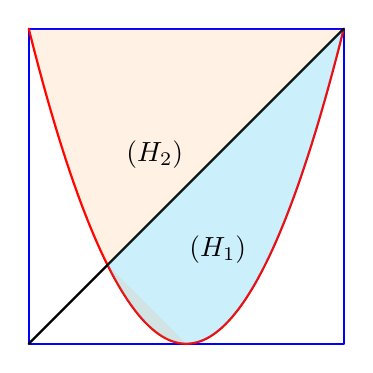
\begin{tikzpicture}[scale=4, line join=round, line cap=round, >=stealth]
			% Vẽ hình vuông
			\draw[thick, blue] (0,0) rectangle (1,1);			
			% Vẽ Parabol: y = 4(x-0.5)^2
			\draw[thick, red, smooth, samples=100, domain=0:1] plot(\x, {4*(\x-0.5)^2});			
			% Vẽ đường chéo y = x
			\draw[thick, black] (0,0) -- (1,1);			
			% Tô màu miền H1 (giới hạn bởi parabol và đường chéo)
			\fill[cyan, opacity=0.2, domain=0.25:1, samples=100] 
			plot(\x, {4*(\x-0.5)^2}) -- (1,1) -- cycle;			
			% Tô màu miền H2 (phần còn lại của parabol)
			\fill[orange, opacity=0.1, domain=0:0.25, samples=100] 
			(0,1) -- plot(\x, {4*(\x-0.5)^2}) -- (0.25,0.25) -- (1,1) -- cycle;
			\fill[orange, opacity=0.1, domain=0.25:0.5, samples=100]
			(0.25,0.25) -- plot(\x, {4*(\x-0.5)^2}) -- (0.5,0) -- cycle;			
			% Kí hiệu H1, H2
			\node at (0.6, 0.3) {$(H_1)$};
			\node at (0.4, 0.6) {$(H_2)$};
		\end{tikzpicture}
	}
	\shortans[oly]{$1{,}4$}
	\loigiai{
		Gọi cạnh hình vuông bằng $1$.\\
		Chọn hệ trục tọa độ $Oxy$ sao cho các đỉnh của hình vuông là $O(0;0)$, $A(1;0)$, $B(1;1)$, $C(0;1)$.\\
		Đường chéo của hình vuông đi qua $O(0;0)$ và $B(1;1)$ có phương trình $y = x$.\\
		Parabol $(P)$ có đỉnh tại trung điểm cạnh đáy $I(0{,}5; 0)$ và đi qua hai đỉnh phía trên $(0;1)$, $(1;1)$.\\
		Phương trình $(P)$ có dạng $y = a(x-0{,}5)^2$. Thay $(0;1)$ vào ta được $1 = a(0-0{,}5)^2 \Rightarrow a=4$.\\
		Vậy phương trình Parabol là $y = 4(x-0{,}5)^2 = 4x^2 - 4x + 1$.\\
		Hoành độ giao điểm của $(P)$ và đường chéo là nghiệm: \[4x^2 - 4x + 1 = x \Leftrightarrow 4x^2 - 5x + 1 = 0 \Leftrightarrow \hoac{& x=1 \\ & x=0{,}25.}\]
		Diện tích phần $(H_1)$ (phần giới hạn bởi đường chéo và Parabol) là
		\[S_1 = \displaystyle\int\limits_{0{,}25}^{1} \big(x - (4x^2 - 4x + 1)\big) \mathrm{\,d}x = \displaystyle\int\limits_{0{,}25}^{1} (-4x^2 + 5x - 1) \mathrm{\,d}x = \dfrac{9}{32}.\]
		Diện tích toàn bộ hình Parabol trong hình vuông là
		\[S_{P} = \displaystyle\int\limits_{0}^{1} \left[1 - (4x^2 - 4x + 1)\right] \mathrm{\,d}x = \dfrac{2}{3}.\]
		Diện tích phần $(H_2)$ là $S_2 = S_P - S_1 = \dfrac{2}{3} - \dfrac{9}{32} = \dfrac{37}{96}$.\\
		Tỉ lệ $\dfrac{S_2}{S_1} = \dfrac{37}{27} \approx 1{,}4$.
	}
\end{ex}
%%%=============================%%%

%%%=============EX_19=============%%%
\begin{ex}%[1H8V5-4]%[TDMZZ05]%[Lê Hồ Quang Minh]
	Cho hình chóp $S.ABC$ có đáy $ABC$ là tam giác đều cạnh bằng $8$, có $SA=SB=12$, hình chiếu vuông góc của đỉnh $S$ trên cạnh $AC$ là điểm $M$ có $MA=3MC$. Hãy tính $\mathrm{d}\big(SC, AB\big)$ \textit{(làm tròn kết quả đến hàng phần trăm)}.
	\shortans[]{$6{,}76$}
	\loigiai{
		\textbf{Cách 1: Dựng mặt phẳng song song}
		\begin{center}
			\begin{tikzpicture}[scale=1, font=\footnotesize, line join=round, line cap=round, >=stealth, declare function={a=6;}]
				\path
				(0,0) coordinate (B)
				(0:a) coordinate (C)
				(60:a) coordinate (A)
				($(A)+(C)-(B)$) coordinate (X)
				($(A)!0.5!(B)$) coordinate (N)
				($(C)!0.3333!(N)$) coordinate (H)
				($(A)!0.75!(C)$) coordinate (M);
				\draw (B)--(C)--(X)--(A)--cycle (C)--(A);
				\draw (A)--(H) (C)--(N) (H)--(M) (N)--(M);
				\draw pic[draw, angle radius=2mm]{right angle=A--N--H};
				\draw pic[draw, angle radius=2mm]{right angle=A--M--H};
				\draw pic[draw, angle radius=5mm]{angle=B--A--C};
				\path (A) ++(-90:22pt) node {$60^\circ$};
				\foreach \p/\pos in {A/90, B/-135, C/-45, X/45, N/135, M/45, H/-90} {
					\fill (\p) circle (1pt) node[shift={(\pos:9pt)}] {$\p$};
				}
			\end{tikzpicture}
			\begin{tikzpicture}[scale=1, font=\footnotesize, line join=round, line cap=round, >=stealth, declare function={a=5; b=2.5; goc=-35; h=4.5;}]
				\path
				(0,0) coordinate (C)
				(0:a) coordinate (B)
				(goc:b) coordinate (A)
				($(A)!0.5!(B)$) coordinate (N)
				($(C)!0.3333!(N)$) coordinate (H)
				($(H)+(90:h)$) coordinate (S);
				\draw[dashed] (C)--(B) (C)--(N) (S)--(H);
				\draw (S)--(C) (S)--(A) (S)--(B) (C)--(A)--(B) (S)--(N);
				\draw pic[draw, angle radius=2mm]{right angle=S--H--N};
				\draw pic[draw, angle radius=2mm]{right angle=S--N--B};
				\foreach \p/\pos in {S/90, A/-90, B/0, C/180, N/-45, H/-135} {
					\fill (\p) circle (1pt) node[shift={(\pos:9pt)}] {$\p$};
				}
			\end{tikzpicture}
		\end{center}
		Gọi $H$ là hình chiếu vuông góc của $S$ lên mặt phẳng $(ABC)$. Gọi $N$ là trung điểm của $AB$.\\
		Vì $SA = SB = 12$ nên $\triangle SAB$ cân tại $S$, suy ra $SN \perp AB$.\\
		Hình chiếu của $SN$ lên mặt phẳng $(ABC)$ là $HN$, nên theo định lý ba đường vuông góc ta có $HN \perp AB$. \\
		Vì $\triangle ABC$ đều nên $N$ là chân đường cao hạ từ $C$. Do đó $H$ nằm trên đường thẳng $CN$.\\
		Mặt khác, theo giả thiết $SM \perp AC$, tương tự ta cũng suy ra được $HM \perp AC$.\\
		Xét tứ giác $AMHN$ có $\widehat{AMH} = 90^\circ$ và $\widehat{ANH} = 90^\circ$.\\
		Suy ra $\widehat{AMH} + \widehat{ANH} = 180^\circ$. Vậy $AMHN$ là tứ giác nội tiếp đường tròn đường kính $AH$.\\
		Xét $\triangle ABC$ đều cạnh $8$, $M \in AC$ thỏa mãn $MA = 3MC \Rightarrow AM = 6$, $MC = 2$.\\
		Xét $\triangle AMN$ có $AM = 6$, $AN = 4$, $\widehat{MAN} = 60^\circ$, theo định lý côsin:
		\[ MN = \sqrt{AM^2 + AN^2 - 2AM \cdot AN \cdot \cos 60^\circ} = 2\sqrt{7}. \]
		Áp dụng định lý sin cho $\triangle AMN$ nội tiếp đường tròn đường kính $AH$, ta có
		\[ AH = \dfrac{MN}{\sin \widehat{MAN}} = \dfrac{2\sqrt{7}}{\sin 60^\circ} = \dfrac{4\sqrt{21}}{3}. \]
		Đường cao của hình chóp là 
		\[ SH = \sqrt{SA^2 - AH^2} = \sqrt{144 - \dfrac{112}{3}} = \dfrac{8\sqrt{15}}{3}. \]
		Trong mặt phẳng $(ABC)$, dựng điểm $X$ sao cho $AXBC$ là hình bình hành.\\
		Khi đó $AB \parallel CX$ nên $AB \parallel (SCX)$. Ta có
		\[ \mathrm{d}\big(AB, SC\big) = \mathrm{d}\big(AB, (SCX)\big) = \mathrm{d}\big(N, (SCX)\big). \]
		Đường cao của đáy $NC = \dfrac{8\sqrt{3}}{2} = 4\sqrt{3}$.\\
		Trong $\triangle AHN$ vuông tại $N$ ta có $NH = \sqrt{AH^2 - AN^2} = \dfrac{8\sqrt{3}}{3}$.\\
		Suy ra $HC = NC - NH = 4\sqrt{3} - \dfrac{8\sqrt{3}}{3} = \dfrac{4\sqrt{3}}{3}$.\\
		Vì $H, C, N$ thẳng hàng nên $\dfrac{\mathrm{d}\big(N, (SCX)\big)}{\mathrm{d}\big(H, (SCX)\big)} = \dfrac{NC}{HC} = 3 \Rightarrow \mathrm{d}\big(N, (SCX)\big) = 3\mathrm{d}\big(H, (SCX)\big)$.\\
		Vì $AXBC$ là hình bình hành nên $CX \perp CN$ hay $CX \perp HC$. \\
		Trong mặt phẳng $(SHC)$, kẻ $HI \perp SC$ tại $I$.\\
		Ta có $\heva{& CX \perp HC \\ & CX \perp SH} \Rightarrow CX \perp (SHC) \Rightarrow CX \perp HI$.\\
		Từ đó $\heva{& HI \perp SC \\ & HI \perp CX} \Rightarrow HI \perp (SCX) \Rightarrow \mathrm{d}\big(H, (SCX)\big) = HI$.\\
		Xét $\triangle SHC$ vuông tại $H$ ta có
		\[ \dfrac{1}{HI^2} = \dfrac{1}{SH^2} + \dfrac{1}{HC^2} = \dfrac{3}{320} + \dfrac{3}{16} = \dfrac{63}{320} \Rightarrow HI = \dfrac{8\sqrt{35}}{21}. \]
		Vậy $\mathrm{d}\big(AB, SC\big) = 3HI = 3 \cdot \dfrac{8\sqrt{35}}{21} = \dfrac{8\sqrt{35}}{7} \approx 6{,}76$.\\
		\textbf{Cách 2: Sử dụng đoạn vuông góc chung}
		\begin{center}
			\begin{tikzpicture}[scale=1.2, font=\footnotesize, line join=round, line cap=round, >=stealth]
				\coordinate (H) at (0,0);
				\coordinate (S) at (0,3.5);
				\coordinate (C) at (1.2,0);
				\coordinate (N) at (-2.8,0);
				\draw (S)--(N)--(C)--cycle (S)--(H);
				\coordinate (K) at ($(S)!(N)!(C)$);
				\draw (N)--(K);
				\draw pic[draw, angle radius=2mm]{right angle=S--H--C};
				\draw pic[draw, angle radius=2mm]{right angle=N--K--S};
				\foreach \p/\pos in {S/90, H/-90, C/-45, N/-135, K/45}
				\fill (\p) circle (1pt) node[shift={(\pos:8pt)}] {$\p$};
			\end{tikzpicture}
		\end{center}
		Gọi $H$ là hình chiếu vuông góc của $S$ lên mặt phẳng $(ABC)$, $N$ là trung điểm của $AB$. \\
		Theo chứng minh ở Cách 1, ta có $H$ thuộc đường thẳng $CN$ và $AB \perp CN$, $AB \perp SH$.\\
		Suy ra $AB \perp (SHC)$. Mà $SC \subset (SHC)$, nên $AB \perp SC$. \\
		Vì $AB \perp (SHC)$ tại $N$, nên khoảng cách giữa hai đường thẳng chéo nhau $AB$ và $SC$ chính là khoảng cách từ điểm $N$ đến đường thẳng $SC$. \\
		Trong mặt phẳng $(SHC)$, kẻ $NK \perp SC$ tại $K$. Khi đó $NK$ chính là đoạn vuông góc chung của $AB$ và $SC$, suy ra $\mathrm{d}(AB, SC) = NK$.\\
		Dựa vào các kết quả tính toán ở Cách 1, ta có
		\begin{itemize}
			\item $SH = \dfrac{8\sqrt{15}}{3}$. 
			\item $NH = \dfrac{8\sqrt{3}}{3}$, $NC = 4\sqrt{3}$ $\Rightarrow HC = \dfrac{4\sqrt{3}}{3}$. 
		\end{itemize}
		Xét $\triangle SHC$ vuông tại $H$, ta có
		\[ SC = \sqrt{SH^2 + HC^2} = \sqrt{\dfrac{320}{3} + \dfrac{16}{3}} = 4\sqrt{7}. \]
		Diện tích tam giác $SNC$ có thể tính theo hai cách
		\[ S_{\triangle SNC} = \dfrac{1}{2} \cdot SH \cdot NC = \dfrac{1}{2} \cdot \mathrm{d}(N, SC) \cdot SC. \]
		Từ đó suy ra
		\[ NK = \mathrm{d}(N, SC) = \dfrac{SH \cdot NC}{SC} = \dfrac{\dfrac{8\sqrt{15}}{3} \cdot 4\sqrt{3}}{4\sqrt{7}} = \dfrac{8\sqrt{35}}{7} \approx 6{,}76. \]
		Vậy $\mathrm{d}\big(AB, SC\big) \approx 6{,}76$.
	}
\end{ex}
%%%=============================%%%

%%%=============EX_20=============%%%
\begin{ex}%[0D8C2-5]%[TDMZZ05]%[Nguyễn Đức Tuấn Anh]
	\immini[thm]{
		Cho tập $X$ là các số nguyên thuộc đoạn $[1;30]$ và $7$ ô tròn $a$, $b$, $c$, $d$, $e$, $f$, $g$ được bố trí như hình vẽ bên dưới. Mỗi ô tròn nhỏ chỉ xếp được đúng một số từ $X$.
		Biết rằng có tất cả $T$ cách chọn ra $7$ số khác nhau từ tập $X$ để xếp vào $7$ ô tròn, sao cho tích của các số xếp trong ba ô tròn thẳng hàng chia hết cho $256$. Hãy tính $\dfrac{T}{100}$ (\textit{làm tròn kết quả đến hàng đơn vị}).}{
		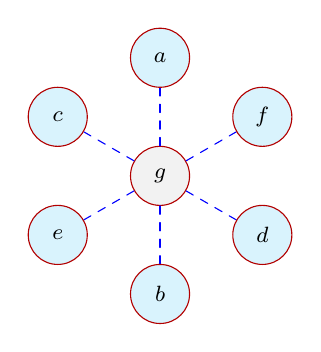
\begin{tikzpicture}[>=stealth, line cap=round, line join=round]
			\tikzset{
				node_base/.style={circle, draw=red!70!black, minimum size=.75cm},
				satellite/.style={node_base, fill=cyan!15}, % Nền xanh nhạt cho các nút vệ tinh
				center_node/.style={node_base, fill=gray!10}, % Nền kem/xám nhạt cho nút trung tâm
				every node/.style={font=\footnotesize}
			}
			\node[center_node] (g) at (0,0) {$g$};
			\def\radius{1.5}
			\foreach \angle/\label in {90/a, 30/f, 330/d, 270/b, 210/e, 150/c} {
				\draw[dashed, blue] (g) -- (\angle:\radius);
				\node[satellite] at (\angle:\radius) {$\label$};
			}
		\end{tikzpicture}
	}
	\par\shortans{$284$}
	\loigiai{
		Từ hình vẽ, ta có $3$ hàng gồm $3$ ô tròn thẳng hàng là $(a, g, b)$, $(c, g, d)$ và $(e, g, f)$.\\
		Tích các số trên mỗi hàng chia hết cho $256 = 2^8$, nên khi phân tích thừa số của $3$ số trên mỗi hàng, tổng số mũ của $2$ trong phân tích phải lớn hơn hoặc bằng $8$.\\
		Gọi $v_2(x)$ là số mũ của $2$ trong phân tích thừa số nguyên tố của $x$. Ta phân nhóm các số trong tập $X = \{1; 2; \dots; 30\}$ theo $v_2(x)$ như sau:
		\begin{itemize}
			\item $P_4 = \{16\}$ (có $1$ số).
			\item $P_3 = \{8; 24\}$ (có $2$ số).
			\item $P_2 = \{4; 12; 20; 28\}$ (có $4$ số).
			\item $P_1 = \{2; 6; 10; 14; 18; 22; 26; 30\}$ (có $8$ số).
			\item $P_0 = \{1; 3; \dots; 29\}$ (có $15$ số).
		\end{itemize}
		Bài toán yêu cầu xếp các số sao cho
		$\heva{&v_2(a) + v_2(g) + v_2(b) \ge 8\\&v_2(c) + v_2(g) + v_2(d) \ge 8\\&v_2(e) + v_2(g) + v_2(f) \ge 8.}$\\
		\textbf{Bước 1: Chứng minh $g = 16$.}\\
		Giả sử $g \ne 16$, khi đó $v_2(g) \le 3$. Để tổng $v_2$ mỗi hàng $\ge 8$, tổng $v_2$ của hai ô còn lại trong mỗi hàng phải $\ge 5$.\\
		Sáu ô còn lại được chọn từ $X \setminus \{g\}$. Giả sử ta chọn $6$ số có $v_2$ lớn nhất có thể: $4$, $3$, $2$, $2$, $2$, $2$ (tổng là $15$).\\
		Ta cần chia $6$ số này thành $3$ cặp sao cho mỗi cặp có tổng $\ge 5$.\\
		Do tổng của $6$ số là $15$ nên $3$ cặp này phải có tổng chính xác là $5$, $5$, $5$.\\
		Tuy nhiên, số $4$ ghép với bất kỳ số nào trong phần còn lại (đều $\ge 2$) sẽ cho tổng $\ge 6$. Khi đó tổng hai cặp còn lại $\le 15 - 6 = 9$, suy ra sẽ có ít nhất một cặp có tổng $\le 4 < 5$ (không thỏa mãn).\\
		Vậy bắt buộc $g = 16 \Rightarrow v_2(g) = 4$.\\
		\textbf{Bước 2: Đếm số cách xếp khi $g=16$.}\\
		Khi $g=16$, ta cần xếp $6$ ô còn lại thành $3$ cặp sao cho tổng $v_2$ của mỗi cặp $\ge 4$.\\
		Vì không còn số nào có $v_2=4$, và chỉ có hai số có $v_2=3$, ta không thể dùng các số thuộc $P_0$ (vì $0+3 < 4$). Do đó $6$ số phải được chọn từ $P_3 \cup P_2 \cup P_1$.\\
		Ta chia các trường hợp dựa vào số lượng số thuộc $P_1$ được chọn (mỗi số $P_1$ bắt buộc phải ghép với một số $P_3$ để có tổng $\ge 1+3=4$):
		\begin{enumerate}[\it TH 1:]
			\item Chọn $0$ số thuộc $P_1$.\\
			Ta phải chọn đúng $6$ số từ $P_3 \cup P_2$ (gồm hai số $P_3$ và bốn số $P_2$).\\
			Bất kỳ cách ghép cặp nào cũng thỏa mãn vì giá trị nhỏ nhất của cặp là từ hai số $P_2$ ($2+2=4 \ge 4$).\\
			Số cách xếp là số hoán vị của $6$ số này vào $6$ vị trí: $6! = 720$ cách.
			\item Chọn $1$ số thuộc $P_1$.\\
			Số cách chọn $1$ số thuộc $P_1$ là $8$ cách. Số này phải ghép cặp với $1$ số thuộc $P_3$.\\
			Ta cần chọn $5$ số nữa từ $6$ số của $P_3 \cup P_2$, tức là loại ra $1$ số:
			\begin{itemize}
				\item \textit{Loại $1$ số thuộc $P_3$ (có $2$ cách):} $6$ số được xếp gồm $1$ số $P_1$, $1$ số $P_3$ và $4$ số $P_2$. Cặp $(P_1, P_3)$ có $3$ cách chọn đường thẳng, có $2!$ cách xếp vào đường đó. $4$ số $P_2$ xếp vào $4$ ô còn lại có $4!$ cách.\\
				Số cách: $8 \cdot 2 \cdot 3 \cdot 2! \cdot 4! = 2\,304$ cách.
				\item \textit{Loại $1$ số thuộc $P_2$ (có $4$ cách):} $6$ số được xếp gồm $1$ số $P_1$, $2$ số $P_3$ và $3$ số $P_2$.\\
				Số $P_1$ xếp vào $1$ trong $6$ ô (có $6$ cách). Ô đối diện phải là $1$ số $P_3$ (có $2$ cách chọn $P_3$). $4$ số còn lại xếp vào $4$ ô có $4!$ cách.\\
				Số cách: $8 \cdot 4 \cdot 6 \cdot 2 \cdot 4! = 9\,216$ cách.
			\end{itemize}
			Tổng cộng TH 2 có $2\,304 + 9\,216 = 11\,520$ cách.
			\item Chọn $2$ số thuộc $P_1$.\\
			Số cách chọn $2$ số thuộc $P_1$ là $\mathrm{C}_8^2 = 28$ cách. Hai số này phải ghép với cả hai số $P_3$.\\
			Chọn thêm $2$ số $P_2$ để đủ $6$ số (có $\mathrm{C}_4^2 = 6$ cách).\\
			Cặp hai số $P_2$ chọn $1$ trong $3$ đường và xếp vào (có $3 \cdot 2! = 6$ cách).\\
			Hai số $P_1$ xếp vào $4$ ô còn lại: chọn $1$ ô cho số thứ nhất (có $4$ cách), số thứ hai phải khác đường nên có $2$ cách. Tổng $4 \cdot 2 = 8$ cách.\\
			Hai số $P_3$ xếp vào $2$ ô đối diện của $P_1$ có $2! = 2$ cách.\\
			Số cách: $28 \cdot 6 \cdot 6 \cdot 8 \cdot 2 = 16\,128$ cách.
		\end{enumerate}
		Tổng số cách thỏa mãn là $T = 720 + 11\,520 + 16\,128 = 28\,368$ cách.\\
		Ta có $\dfrac{T}{100} = \dfrac{28\,368}{100} \approx 284$.
	}
\end{ex}
%%%=============================%%%

%%%=============EX_21=============%%%
\begin{ex}%[2D1C3-5]%[TDMZZ05]%[Nguyễn Văn Sang]
	\immini[thm]
	{Cho ba thanh cứng $AB$, $BC$, $CD$ gắn với nhau bằng hai bản lề tại $B$ và $C$, hai đầu còn lại được gắn cố định với sàn nhà tại hai bản lề $A$ và $D$. Biết rằng $AB = 4$ m, $BC = CD = 3$ m, $AD = 7$ m, mặt phẳng $(ABCD)$ luôn vuông góc với sàn nhà. Khi hai bản lề $B$ và $C$ di chuyển thì điểm $B$ cách sàn nhà một khoảng lớn nhất bằng bao nhiêu milimet \textit{(làm tròn kết quả đến hàng đơn vị)}?
	}
	{\begin{tikzpicture}[scale=0.8, >=stealth]
			\coordinate (D) at (0,0);
			\coordinate (A) at (7,0);
			
			% Góc giả định để vẽ minh họa giống đề bài
			\def\angleC{55}
			\coordinate (C) at (\angleC:3);
			
			% Tìm điểm B qua giao tuyến 2 đường tròn
			\path[name path=circleC] (C) circle (3);
			\path[name path=circleA] (A) circle (4);
			\path [name intersections={of=circleC and circleA, by={B, B2}}];
			
			% Vẽ mặt sàn
			\draw (-1.5,0) -- (9,0) node[above] {Sàn nhà};
			
			% Vẽ các thanh cứng
			\draw[red!80!black, thick] (D) -- (C) node[midway, left] {$3\text{m}$};
			\draw[red!80!black, thick] (C) -- (B) node[midway, below=2pt] {$3\text{m}$};
			\draw[blue, thick] (B) -- (A) node[midway, right] {$4\text{m}$};
			
			% Vẽ các khớp nối
			\fill[blue] (C) circle (2pt) node[above] {\color{black}$C$};
			\fill[blue] (B) circle (2pt) node[above right] {\color{black}$B$};
			\fill[blue] (D) circle (2pt) node[below left=2pt] {\color{black}$D$};
			\fill[blue] (A) circle (2pt) node[above right=2pt] {\color{black}$A$};
			
			\node[below right, align=center] at (D) {Cố định};
			\node[below, align=center] at (A) {Cố định};
	\end{tikzpicture}}
	\par\shortans[0]{$3422$}
	\loigiai{
		\begin{center}
			\begin{tikzpicture}[scale=0.79, >=stealth]
				\coordinate (D) at (0,0);
				\coordinate (A) at (7,0);
				
				% Thêm 'overlay' để 2 đường tròn tàng hình này KHÔNG làm phình to Bounding Box
				\path[name path=circleD, overlay] (D) circle (6);
				\path[name path=circleA, overlay] (A) circle (4);
				\path [name intersections={of=circleD and circleA, by={B, B2}}];
				
				% C là trung điểm của BD do BC = CD = 3
				\coordinate (C) at ($(D)!0.5!(B)$);
				\coordinate (H) at (B|-D);
				
				% Vẽ sàn nhà
				\draw (-1.5,0) -- (9,0) node[above] {Sàn nhà};
				
				% Vẽ các thanh ở cấu hình tối đa
				\draw[red!80!black, thick] (D) -- (C) node[midway, above left] {$3\text{m}$};
				\draw[red!80!black, thick] (C) -- (B) node[midway, above left] {$3\text{m}$};
				\draw[blue, thick] (B) -- (A) node[midway, right=2pt] {$4\text{m}$};
				
				% Vẽ đường cao h_max
				\draw[dashed, thick] (B) -- (H) node[midway, left] {$h_{\max}$};
				\draw (H) ++(0,0.25) -- ++(-0.25,0) -- ++(0,-0.25);
				\node[below] at (H) {$H$};
				
				% Vẽ các khớp nối
				\fill[blue] (C) circle (2.5pt);
				\fill[blue] (B) circle (2.5pt);
				\fill[blue] (D) circle (2.5pt);
				\fill[blue] (A) circle (2.5pt);
				\node[above left] at (C) {$C$};
				\node[above] at (B) {$B$};
				\node[below left] at (D) {$D$};
				\node[below right] at (A) {$A$};
			\end{tikzpicture}
		\end{center}
		Kẻ đường cao $BH \perp AD$ tại $H$. Khi đó khoảng cách từ $B$ đến sàn nhà là $h = BH$.\\
		Xét $\triangle BCD$, theo bất đẳng thức tam giác ta luôn có
		\[ BD \le BC + CD = 3 + 3 = 6 \text{ (m)}.\]
		Dấu ``$=$'' xảy ra khi $C$ nằm giữa $B$ và $D$, tức là $3$ điểm $D, C, B$ thẳng hàng và thanh $CD$, $BC$ được duỗi thẳng tối đa.
		Mặt khác, xét $\triangle ABD$, ta có $BD \ge |AD - AB| = |7 - 4| = 3$.\\
		Vậy độ dài $x = BD$ luôn nằm trong đoạn $[3; 6]$.\\
		Áp dụng công thức Heron để tính diện tích $\triangle ABD$ với ba cạnh là $AB=4, AD=7, BD=x$.\\
		Nửa chu vi $p = \dfrac{7 + 4 + x}{2} = \dfrac{11 + x}{2}$.\\
		Bình phương diện tích tam giác là
		\begin{eqnarray*}
			S_{ABD}^2 &=& p(p - 7)(p - 4)(p - x) \\
			&=& \dfrac{11 + x}{2} \cdot \dfrac{x - 3}{2} \cdot \dfrac{x + 3}{2} \cdot \dfrac{11 - x}{2} \\
			&=& \dfrac{1}{16} \left( 121 - x^2 \right) \left( x^2 - 9 \right).
		\end{eqnarray*}
		Đặt $t = x^2$. Vì $x \in [3; 6]$ nên $t \in [9; 36]$.\\
		Ta xét hàm số $f(t) = (121 - t)(t - 9) = -t^2 + 130t - 1089$ trên đoạn $[9; 36]$.\\
		Đạo hàm $f'(t) = -2t + 130$. Cho $f'(t) = 0 \Leftrightarrow t = 65 \notin [9; 36]$.\\
		Với mọi $t \in [9; 36]$ ta thấy $f'(t) > 0$. Ta có bảng biến thiên
		\begin{center}
			
\begin{tikzpicture}
				\tkzTabInit[lgt=1.5,espcl=5,nocadre=false, deltacl=0.65]
				{$t$ /1, $f'(t)$ /1, $f(t)$ /2}
				{$9$, $36$}
				\tkzTabLine{, +, }
				\tkzTabVar{-/ $0$, +/ $2\,295$}
			\end{tikzpicture}
		\end{center}
		Dựa vào bảng biến thiên, ta suy ra $\max\limits_{[9; 36]} f(t) = f(36) = 2\,295$.
		Khi đó, diện tích tam giác $ABD$ đạt giá trị lớn nhất là
		\[ S_{ABD(\max)} = \sqrt{\dfrac{2\,295}{16}} = \dfrac{3\sqrt{255}}{4} \left(\text{m}^2\right).\]
		Khoảng cách lớn nhất từ $B$ đến sàn nhà là
		\[ h_{\max} = \dfrac{2 \cdot S_{ABD(\max)}}{AD} = \dfrac{2 \cdot \dfrac{3\sqrt{255}}{4}}{7} = \dfrac{3\sqrt{255}}{14} \text{ (m)}.\]
		Đổi đơn vị sang milimet
		\[ h_{\max} = \dfrac{3\sqrt{255}}{14} \times 1\,000 = \dfrac{1\,500\sqrt{255}}{7} \approx 3\,422 \text{ (mm)}.\]
	}
\end{ex}
%%%=============================%%%

%%%=============EX_22=============%%%
\begin{ex}%[0D0C2-3]%[TDMZZ05]%[Nguyễn Thành Hậu]
	Xếp ngẫu nhiên $4$ học sinh lớp $A$ và $4$ học sinh lớp $B$ vào $20$ ghế hàng ngang.
	Gọi $p$ là xác suất để mỗi lớp đứng thành một cụm (tức là $4$ học sinh mỗi lớp đứng cạnh nhau),
	nếu biết có ít nhất một trong hai lớp các em học sinh đã đứng thành một cụm.
	Hãy tính $10^5 p$ (\textit{làm tròn kết quả đến hàng đơn vị}).
	\par
	\shortans[0]{$295$}
	\loigiai{
		Việc lấy hoán vị các học sinh cùng lớp không ảnh hưởng đến xác suất cần tính nên ta bỏ qua (xem các hoán vị là giống nhau).\\
		Đếm số cách xếp sao cho $4$ học sinh lớp $A$ đứng thành cụm:\\
		Xếp $4$ học sinh lớp $A$ cạnh nhau trên hàng ghế $20$ vị trí có $17$ cách. Xếp $4$ học sinh lớp $B$ vào $16$ chỗ còn lại có $\mathrm{C}_{16}^{4}$ cách. Do đó, có tất cả $17\mathrm{C}_{16}^{4}$ cách.\\
		Tương tự, số cách xếp sao cho $4$ học sinh lớp $B$ đứng thành cụm cũng bằng $17\mathrm{C}_{16}^{4}$.\\
		Đếm số cách xếp mà các học sinh cùng lớp đứng thành cụm:\\
		Giả sử xếp $4$ học sinh lớp $A$ vào các vị trí $k$, $k+1$, $k+2$, $k+3$. \\
		Nếu $1\le k\le 4$ thì $4$ học sinh lớp $B$ chỉ có thể xếp vào các vị trí từ $k+4$ trở đi, có $20-(k+4)+1=17-k$ vị trí trống nên có $14-k$ cách xếp học sinh lớp $B$ thành một cụm.\\
		Nếu $17\le k+3\le 20$ hay $14\le k\le 17$, tương tự như trên cũng có $k-4$ cách xếp học sinh lớp $B$ thành cụm.\\
		Nếu $5\le k\le 13$ thì có $(k-4)+(14-k)=10$ cách xếp các học sinh lớp $B$ thành cụm.
		Do đó số cách xếp mà các học sinh cùng lớp đứng thành cụm là \[\sum_{k=1}^{4}(14-k)+\sum_{k=14}^{17}(k-4)+\sum_{k=5}^{13}10=182.\]
		Theo nguyên lý bù trừ, số cách xếp mà có ít nhất một trong hai lớp các em học sinh đã đứng thành một cụm là \[2\cdot 17\mathrm{C}_{16}^{4}-182.\]
		Khi đó, \[p=\dfrac{182}{2\cdot 17\mathrm{C}_{16}^{4}-182}\Rightarrow 10^{5}p=\dfrac{182\cdot 10^{5}}{2\cdot 17\mathrm{C}_{16}^{4}-182}\approx 295.\]
		\textbf{Cách khác} ta có thể đếm số cách xếp mà các học sinh cùng lớp đứng thành cụm như sau.\\
		Gọi $x$, $y$, $z$ là số vị trí trống do hai cụm học sinh của hai lớp tạo ra, khi đó
		\[\heva{&x,y,z\in\mathbb{N}\\
			&x+y+z=12.}\]
		Sử dụng bài toán chia kẹo Euler, có $\mathrm{C}_{12+3-1}^{3-1}=\mathrm{C}_{14}^{2}=91$ bộ $(x,y,z)$. Với mỗi bộ $(x,y,z)$ có hai cách xếp (hoán vị hai cụm học sinh), nên có $2\cdot \mathrm{C}_{14}^{2}=182$ cách xếp.
	}
\end{ex}
%%%=============================%%%
